%!TEX root = ../main.tex
%%%%%%%%%%%%%%%%%%%%%%%%%%%%%%%%%%
% Links: https://medium.com/@hazemu/finding-the-median-of-2-sorted-arrays-in-logarithmic-time-1d3f2ecbeb46
%
% Difficulty: Companies: 
%%%%%%%%%%%%%%%%%%%%%%%%%%%%%%%%%%

\chapter{Median of two sorted arrays}
\label{ch:median_sorted_arrays}
\section*{Introduction}

The median is one of the most basic and important concept in statistics and probability theory and
it finds applications in almost every field of science. It is defined as the value that split a
certain data set into two equally sized halves: the higher and the lower half. For example the median of the
dataset $\{1,3,4,6,10,12,19\}$ is $6$ because we have $3$ elements greater and $3$ elements smaller
than $6$. When the size of the dataset is even, such element does not exists and thus the median is defined as the mean of the two middle elements;
For instance given the dataset $\{1,3,4,6,8,10,12,19\}$, the median is $\frac{6+8}{2}=7$.  

The problem covered in this chapter is about finding the median from a dataset provided as two
separate input list of values (you can imagine, for instance, that each of the input set comes from
a separate thread as part of a multithreaded application to analyze a large dataset).
Despite an obvious solution exists that pretty follows from the definition of
median, this problem is considered to be hard to solve optimally in a coding interview context
as it requires non-trivial insights and careful implementation.
But, despite its daunting reputation has been asked often during coding interviews.

For the rest of the chapter we will go throught the problem statement, and then we dive deeper into the
problem by discussing a number of possible approaches that will make us go from a naive and
inefficient to a more sophisticated but optimal solution. 

\section{Problem statement}
\begin{exercise}
You are given two \textbf{sorted} arrays $A$ and $B$ of size $m$ and $n$, respectively. Your task is
to write a function that takes as input $A$ and $B$ and returns the median of the two sorted arrays.
$A$ and $B$ con be considered to be proper subsets of a third dataset $C = A \cup B$. 

	\begin{example}
		\hfill \\
		Given two sorted arrays:
		\begin{itemize}
			\item $A=[1,4,6,10,15]$
			\item $B=[2,3,5,6]$
		\end{itemize}
		The median is $5$ (see Figure \ref{fig:median_sorted_arrays:example2}).
	\end{example}

	\begin{example}
		\hfill \\
		Given two sorted arrays:
		\begin{itemize}
			\item $A=[1,4,6,10]$
			\item $B=[2,3,5,6]$
		\end{itemize}
		The median is $\frac{5+4}{2} = 4.5$ (see Figure \ref{fig:median_sorted_arrays:example1}).
	\end{example}

\end{exercise}

\begin{figure}
	\label{fig:median_sorted_arrays:example2}
	\centering
	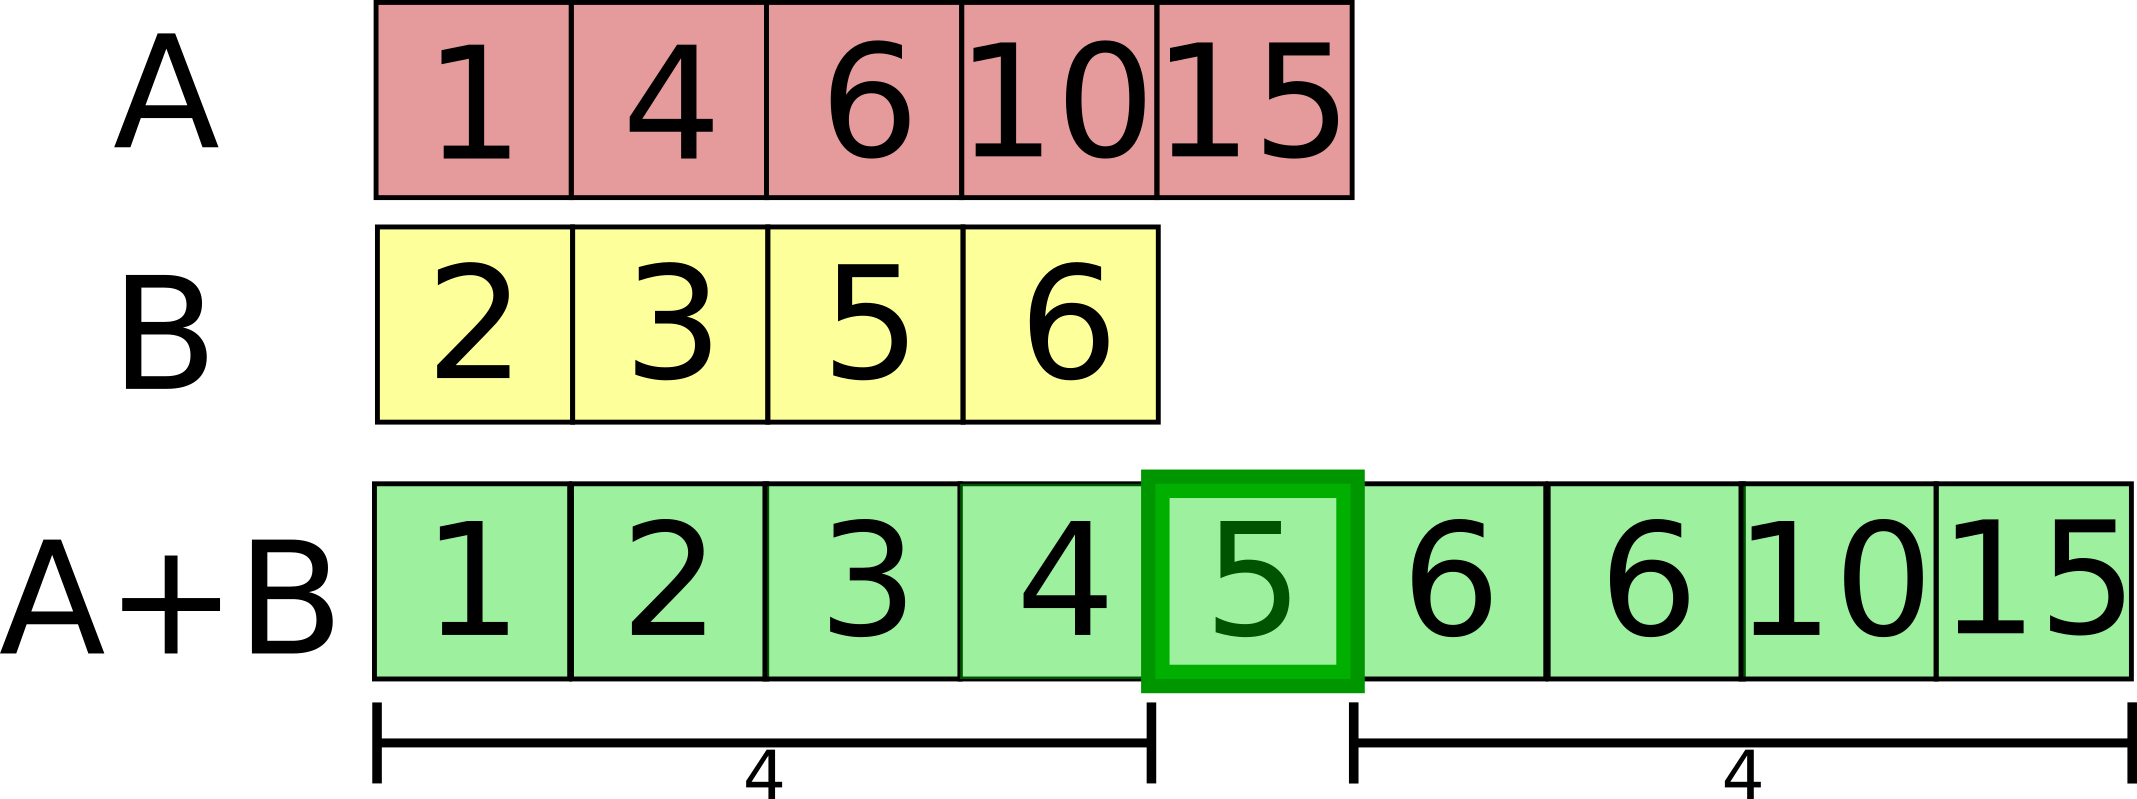
\includegraphics[scale=1.0]{sources/median_sorted_arrays/images/example2}
	\caption[Example of median of two sorted array.]{Example of median of two sorted array where the total number of elements is odd.}
\end{figure}

\begin{figure}
	\label{fig:median_sorted_arrays:example1}
	\centering
	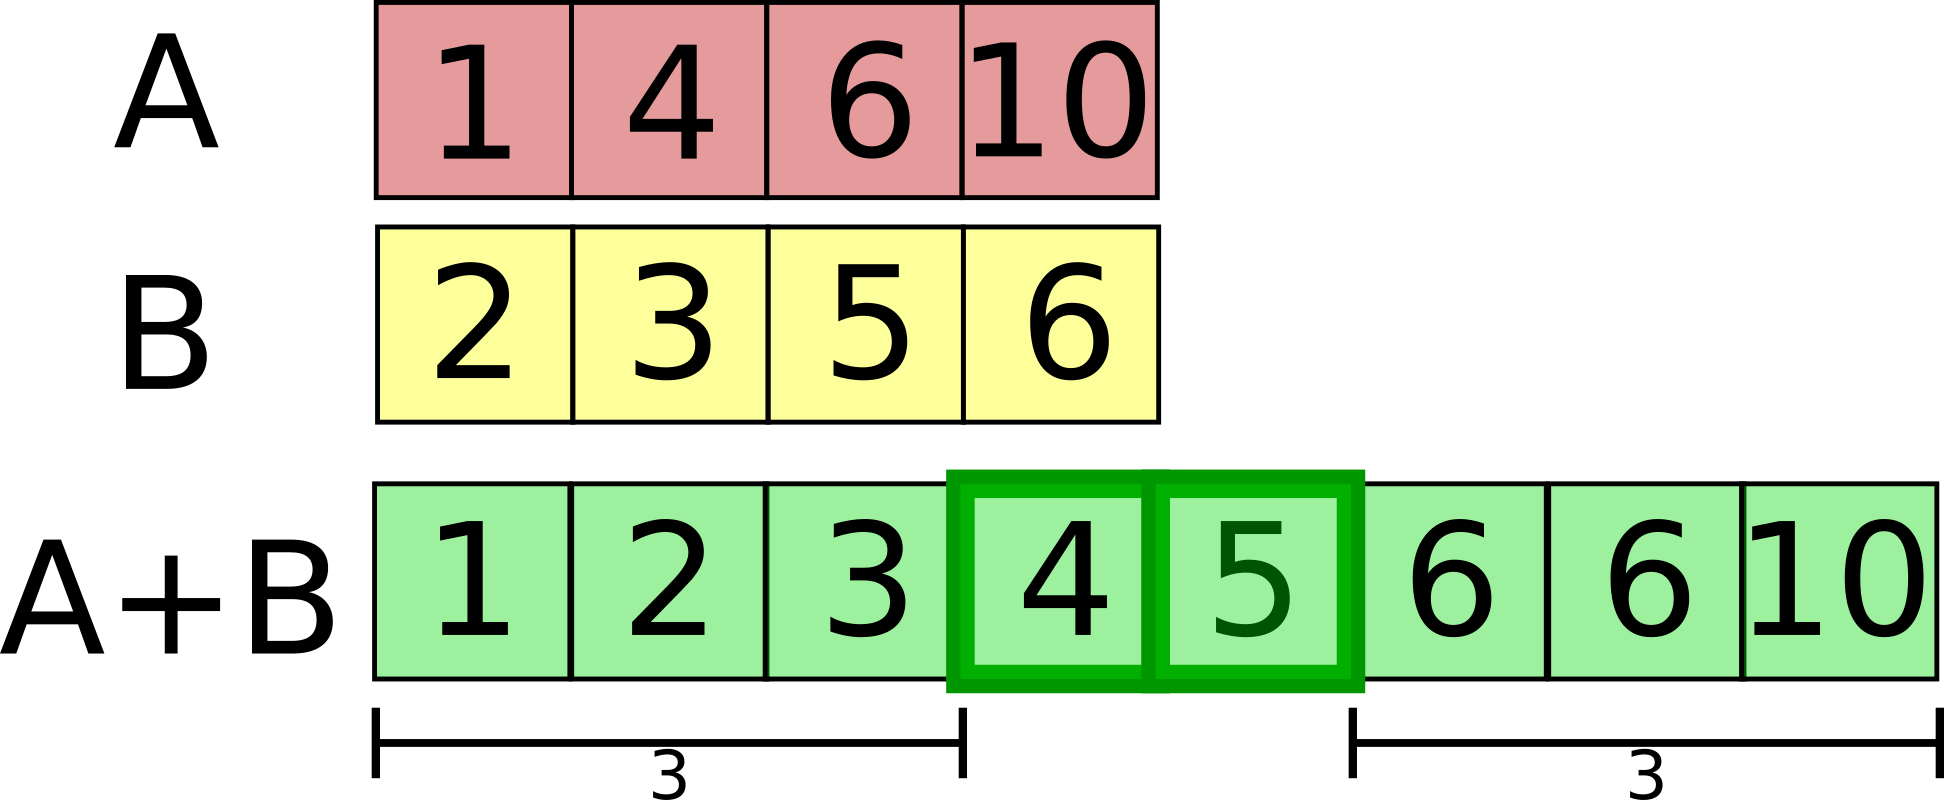
\includegraphics[scale=1.0]{sources/median_sorted_arrays/images/example1}
	\caption[Example of median of two sorted array.]{Example of median of two sorted array where the total number of element is even.}
\end{figure}


\section{Clarification Questions}

\begin{QandA}
	\item Can $A$ or $B$ be empty?
	\begin{answered}
		\textit{Yes, but you can assume that $|A \cup B| > 0$ i.e. at most one of the input array can be empty.}
	\end{answered}
	
\end{QandA}

\section{Discussion}
\label{median_sorted_arrays:sec:discussion}
Let's start our discussion by reviewing the concept of median. The median of a collection $C$ of $n$
elements is ($C_i$ represents the $i^{th}$ element of $C$):
\begin{itemize}
	\item $C_{\frac{n}{2}}$ if $n$ is odd (see Figure \ref{fig:median_sorted_arrays:example1})
	\item $\frac{C_{ \lfloor \frac{n}{2} \rfloor    }+C_{ \lceil \frac{n}{2} \rceil   }}{2}$ if $n$ is even (see Figure
	\ref{fig:median_sorted_arrays:example2})
\end{itemize}
In simpler terms the median of a sorted collection is the element which divides the collections into
two equally sized halves, left and right, each with the same number of elements. 
If $n$ is even, clearly such element does not exists and thus the median is the defined to be the mean of the two middle
elements as shown in Figure \ref{fig:median_sorted_arrays:example1}.
Additionally, notice that because the collection is sorted then all the elements in the left half are smaller or equal then
the median and all the elements on the right half are larger. 

\subsection{Brute-force}
\label{median_sorted_arrays:sec:bruteforce}
Armed with the definition of median, we can immediately devise a simple and effective approach to
find it given the two input sorted arrays. The only difference between the problem statement and the
definition of median is that we are given two sorted arrays and not just one. Therefore it is
natural that the very first thing that should come to mind is to:
\begin{enumerate}
	\item create a third array $C = A \cup B$, which is the concatenation of the two input arrays
	\item proceed by sorting $C$,
	\item calculate the median (and not forgetting to take into consideration the parity of $|C|$)
\end{enumerate}

This approach is clearly correct as it is basically a direct consequence and application of the
definition of median given above, but it is far from being optimal, as we will see below. Listing
\ref{list:median_sorted_naive} shows a C++ implementation of this idea. Time and space complexities
of this approach are $O((n+m)log(n+m))$(because of sorting) and $O(s+m)$(space required by the third
array), respectively. Despite being suboptimal this solution has the benefit of being very short (only a few lines)
and easy to read, explain and understand.

\lstinputlisting[language=c++, caption={Naive implementation of solution to the problem of finding the median of two sorted arrays.},label=list:median_sorted_naive]{sources/median_sorted_arrays/median_sorted_arrays_solution1.cpp}


\subsection{Brute-force improved}
\label{median_sorted_arrays:sec:bruteforce_improved}
The brute-force approach can be improved a bit if we use the fact that the arrays are already
sorted. In the approach described in Section \ref{median_sorted_arrays:sec:bruteforce} we do not use
this fact and therefore we are forced to sort the entire array $C$ that we created by blindly juxtaposing $A$ and $B$ one after the other.
By taking advantage of the fact that the inputs are sorted we can create the array $C$ in a smarter way,
so that it is already sorted. In order to do so we will use the fact that you can merge two sorted array into a third sorted array in linear time.
You might be already familiar with this idea if you know how the famous merge-sort algorithm\cite{wiki:mergesort} works as the same operation is one of its two basic building blocks.
Listing \ref{list:median_sorted_naive_2} shows how this idea can be coded in C++. Notice how most of the code is now taken by the \inline{std::vector<T> mergeSortedArrays(const std::vector<T> &A,
const std::vector<T> &B)} function that 
is responsible for taking two sorted arrays (pay attention to the \inline{assert}) as input and returning a third sorted one. 

\lstinputlisting[language=c++, caption={Naive implementation of solution to the problem of finding the median of two sorted arrays using the merge part of merge-sort algorithm.},label=list:median_sorted_naive_2]{sources/median_sorted_arrays/median_sorted_arrays_solution2.cpp}

The time and complexities of this version are both $O(n+m)$, much better than the one from the solution presented in
Section \ref{median_sorted_arrays:sec:bruteforce} but, it is still suboptimal as this problem can be
solved in logarithmic time. We are going to see how in Section \ref{median_sorted_arrays:sec:log}.

\subsubsection{Merge sorted arrays in linear time}
How exactly can we merge two sorted arrays $X$ and $Y$ into a third sorted array $Z$ in linear time? 
The idea behind is that we can build $Z$ incrementally starting from an empty array, and at each step of the process
inserting one of the elements of $X$ or $Y$ depening on which one of the two containts the smallest element at that moment.
In the implementation of \inline{mergeSortedArrays} this is achieved by using two iterators, \inline{itX} and \inline{itY} 
each pointing to the next element of $X$ and $Y$ to be inserted in $Z$, respectively.
The \inline{while} loop is responsible for comparing the two elements pointed by the iterators and always inserting the smallest one
into $Z$.  Once an element is merged in the final array, the corrensponding iterator is incremented so the next value will be considered at the next iteration.
When one of the two iterators its the end of its array, then all we are left are the remaining elements of the other collection that we can at this point blindly insert into $Z$ because they are sorted 
(see the last two \inline{while} loops in the code).
Figure \ref{fig:median_sorted_array:mergearray} shows all the steps that are necessary to perform the merging for the arrays:
$X = \{1,3,5,8,15\}$ and $X = \{2,4,7\}$. At step $1$ (Figure \ref{fig:median_sorted_array:mergearray0}) $Z$ is initially empty and \inline{itA} and \inline{itB} point to the beginning of $X$ and $Y$, respectively.
Because the element pointed by itA is smaller, it is selected for merging and thus itA is incremented.
At step $2$ (Figure \ref{fig:median_sorted_array:mergearray1}) the element pointed by itB is smaller, and as in the previous step, it is merged in $Z$ and itB is incremeneted.
The same operations are performed for all the steps depicted in Figures 
\ref{fig:median_sorted_array:mergearray2},
\ref{fig:median_sorted_array:mergearray3},
\ref{fig:median_sorted_array:mergearray4},
\ref{fig:median_sorted_array:mergearray5} and \ref{fig:median_sorted_array:mergearray6}.
Eventually itB goes out of range signalling that all the element in $Y$ have been processed (see Figure \ref{fig:median_sorted_array:mergearray6}).
At this point then, as shown in Figure \ref{fig:median_sorted_array:mergearray7} we can safely merge all the element in $X$ into $Z$ that is now ready to be returned (see Figure \ref{fig:median_sorted_array:mergearray8}).

\begin{figure}
	\centering
	\begin{subfigure}[b]{0.45\textwidth}
		\centering
		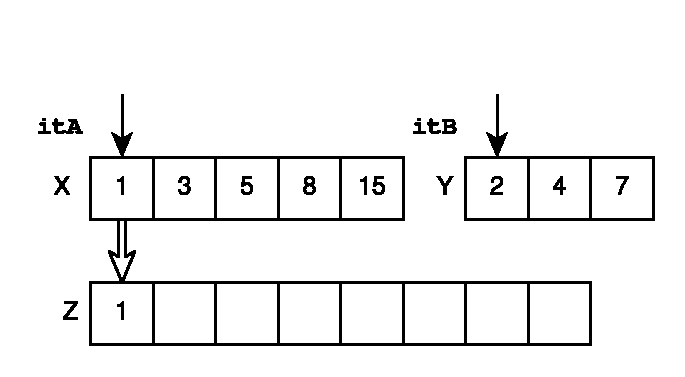
\includegraphics[trim=0 0 0 45,clip,width=\textwidth]{sources/median_sorted_arrays/images/mergearrays0}
		\caption{Step $1$: $Z$ is initially empty. itX and itY points to the beginning of $X$ and $Y$, respectively. The element pointed by itX is merged as it is smaller. itX is advanced by one position.}
		\label{fig:median_sorted_array:mergearray0}
	\end{subfigure}
	\hfill
	\begin{subfigure}[b]{0.45\textwidth}
		\centering
		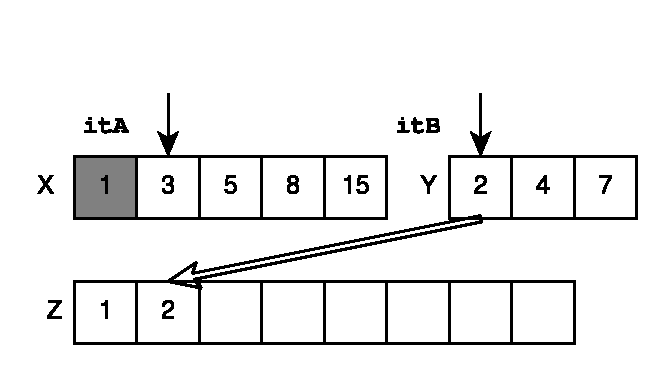
\includegraphics[trim=0 0 0 45,clip,width=\textwidth]{sources/median_sorted_arrays/images/mergearrays1}
		\caption{Step $2$: itY is smaller than itX, thus it is the one being merged. itB is also advanced by one position. }
		\label{fig:median_sorted_array:mergearray1}
	\end{subfigure}
	\hfill

	\begin{subfigure}[b]{0.45\textwidth}
		\centering
		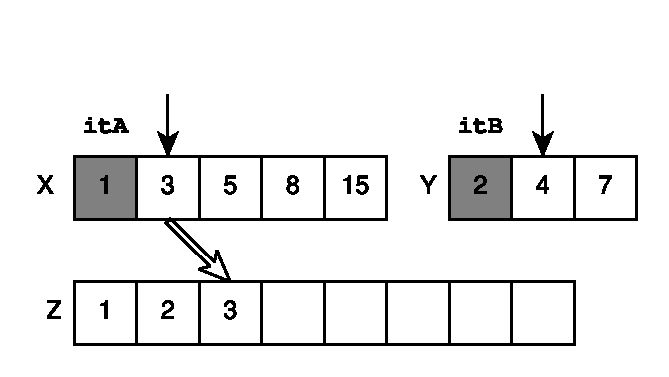
\includegraphics[trim=0 0 0 45,clip,width=\textwidth]{sources/median_sorted_arrays/images/mergearrays2}
		\caption{Step $3$: itX is smaller than itY, thus it is the one being merged. itX is also advanced by one position.}
		\label{fig:median_sorted_array:mergearray2}
	\end{subfigure}
	\hfill
	\begin{subfigure}[b]{0.45\textwidth}
		\centering
		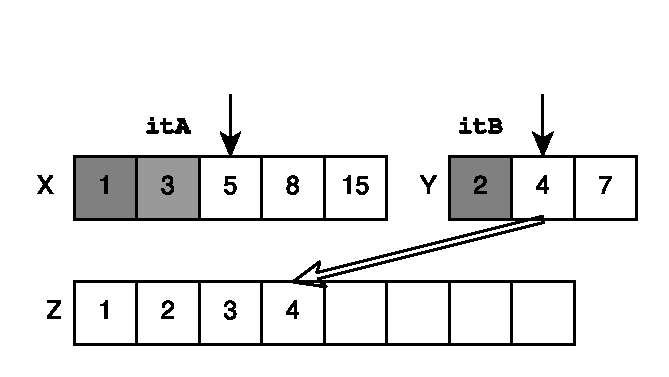
\includegraphics[trim=0 0 0 45,clip,width=\textwidth]{sources/median_sorted_arrays/images/mergearrays3}
		\caption{Step $4$: itY is smaller than itX, thus it is the one being merged. itB is also advanced by one position. }
		\label{fig:median_sorted_array:mergearray3}
	\end{subfigure}
	\hfill

	\begin{subfigure}[b]{0.45\textwidth}
		\centering
		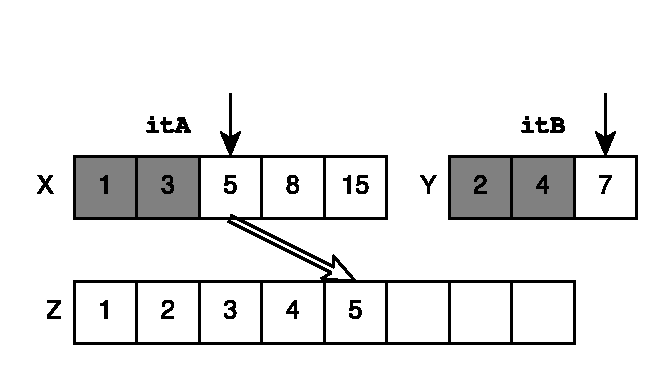
\includegraphics[trim=0 0 0 45,clip,width=\textwidth]{sources/median_sorted_arrays/images/mergearrays4}
		\caption{Step $5$:  itX is smaller than itY, thus it is the one being merged. itX is also advanced by one position.}
		\label{fig:median_sorted_array:mergearray4}
	\end{subfigure}
	\hfill
	\begin{subfigure}[b]{0.45\textwidth}
		\centering
		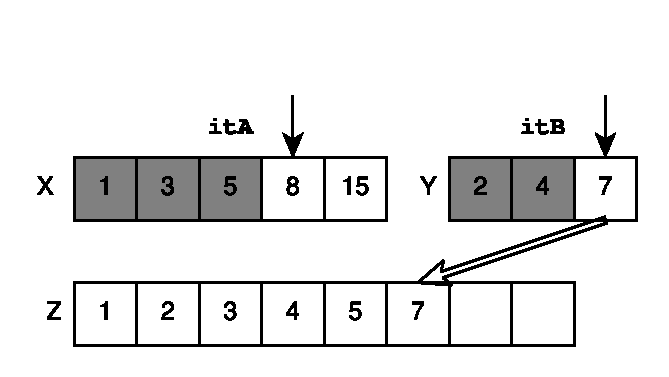
\includegraphics[trim=0 0 0 45,clip,width=\textwidth]{sources/median_sorted_arrays/images/mergearrays5}
		\caption{Step $6$:itY is smaller than itX, thus it is the one being merged. itB is also advanced by one position.}
		\label{fig:median_sorted_array:mergearray5}
	\end{subfigure}
	\hfill

	\begin{subfigure}[b]{0.45\textwidth}
		\centering
		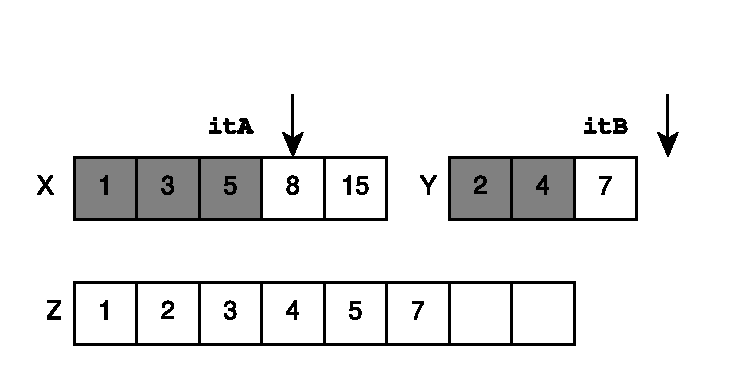
\includegraphics[trim=0 0 0 45,clip,width=\textwidth]{sources/median_sorted_arrays/images/mergearrays6}
		\caption{ itY now  points to the past-the-end element of $Y$. There are no more element of $Y$ to merge.}
		\label{fig:median_sorted_array:mergearray6}
	\end{subfigure}
	\hfill
	\begin{subfigure}[b]{0.45\textwidth}
		\centering
		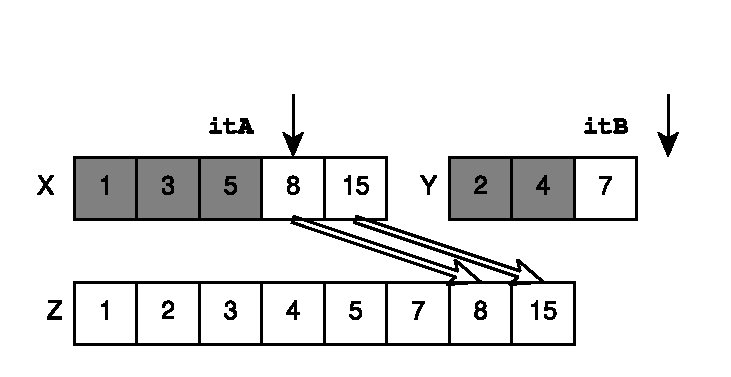
\includegraphics[trim=0 0 0 45,clip,width=\textwidth]{sources/median_sorted_arrays/images/mergearrays7}
		\caption{Step $7$: All the remaning element from the current location of itX to the end of X are merged into $Z$. }
		\label{fig:median_sorted_array:mergearray7}
	\end{subfigure}
	\hfill
	\begin{subfigure}[b]{0.45\textwidth}
		\centering
		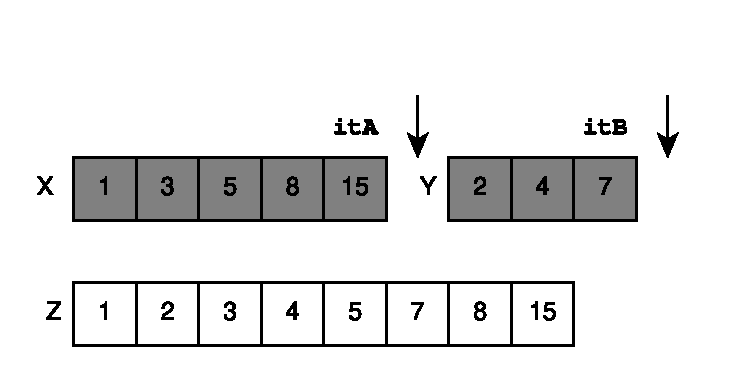
\includegraphics[trim=0 0 0 45,clip,width=\textwidth]{sources/median_sorted_arrays/images/mergearrays8}
		\caption{All the elements of $X$ and $Y$ have been merged. $Z$ contains the element of $X \cup Y$ and it is sorted.}
		\label{fig:median_sorted_array:mergearray8}
	\end{subfigure}
	\caption[Example of merging two sorted arrays.]{This figure shows how two sorted arrays can be merged into a third sorted array in linear time. The hollow indicates which element at that step is selected to go into the third array. Notice that the iterator associated with that element is then moved forward. Already merged cells are }
	\label{fig:median_sorted_array:mergearray}
\end{figure}


\subsection{Logarithmic solution}
\label{median_sorted_arrays:sec:log}
If we want to improve the $O(n+m)$ solution we have at hand at this point we need to abandon the idea of constructing a third array containing all the elements from the inputs.
There is no way this can be done in less than linear time as one must at least access the input element once.
Turns out, we do not actually need to have the array $C$ at all. 

The key insights are:
\begin{itemize}
	\item we know exactly what the size of the merged array $C$ would be: $n+m$.
	\item we also know that the part of $C$ to the left of the median, $C_l$ would be made up from elements among the smallest values of $A$
	and $B$. These values also lie in the left portions of $A$ and $B$. For instance, w.r.t. the example in Figure \ref{fig:median_sorted_arrays:example2} we
	can see that the left half (the first $5$ elements) of $A \cup B$ is made from the first two elements
	of $A$ and the smallest $3$ elements of $B$. Because $C$ will be sorted, only the smallest
	elements of $A$ and $B$ will can be part of $C_l$.
\end{itemize}
The problem is that we do not know exactly how many elements of $A$ will be part $C_l$ but if we do, then, we also know immediately how many elements of $B$ go to $C_l$
and at that point we can calculate the median.
We cannot find directly how many elements  of $A$ contributes to $C_l$, but we can test farily easily if the first $i$ elements do.
Let's suppose we try to make $C_l$ by using $i$ elements from the left portion of $A$.
Because $|C|=n+m$ then $|C_l| = \frac{n+m}{2} = i+j$ where $j$ is the number of elements from the left part of $B$ contributing to $C_l$. 
Thus if we take $i$ elements from $A$ we need to take $j = (n+m)-i$ elements from $B$. 
Once $i$ and $j$ are decided, we also know that the last element of $C_l$, will be the maximum element among the first $i$ elements of $A$ and the first $j$ elements of $B$.
From these arguments follows that the right half of $C$, $C_r$,  contains all the remaining $n-i$ elements of $A$ and $m-j$ of $B$, 
and also that the first element of $C_r$ will be the smallest element among them.
Given:
\begin{itemize}
	\item $M_l$ is the largest elements among the $A[i]$  $B[j]$
	\item $m_r$ is the smallest element among the $A[i+1]$  $B[j+1]$
\end{itemize} 
then if $i$ is indeed the right amount of element from $A$ belonging to $C_l$ then, $M_l \leq m_r$.
If $M_l > m_r$ then we need to understand whether we took too many or too few elements from $A$ to be part of $C_l$. 
We can check this by checking whether  $M_l$ belongs to $B$ or $A$, respectively. 
Thus if $A[i] > B[j]$ we reduce or increase $i$ by doing $r = r-1$. 
Conversely if $A[i] < B[i]$ then $i$ is increased by moving the left boundary of the binary search range: $l = l+1$.

Listing \ref{list:median_sorted_binary} shows an implementation of the idea above.
\lstinputlisting[language=c++, caption={Binary search solution to the \textit{median of two sorted arrays} problem.},label=list:median_sorted_binary]{sources/median_sorted_arrays/median_sorted_arrays_solution3.cpp}



https://leetcode.com/problems/median-of-two-sorted-arrays/ complete this code first
use binary search to find i
l , r is the range of elements of A initially l = 0 r = min(n, (n+m)/2)
i = l+r/2
j = n+m-i
if max among A[i] and B[j] <= min A[i+1],B[j+1] we have a median
otherwise 
if A[i] > B[j] then r = i-1
else l = i+1
